\documentclass[11pt]{standalone}
\usepackage{tikz}

\begin{document}

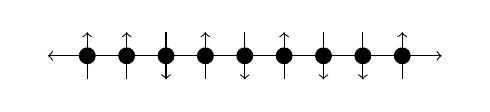
\begin{tikzpicture}

\draw[fill=black] (0,0) circle (.1cm);% node[](9){};
\draw[fill=black] (-0.5,0) circle (.1cm);
\draw[fill=black] (-1.0,0) circle (.1cm);
\draw[fill=black] (-1.5,0) circle (.1cm);
\draw[fill=black] (-2.0,0) circle (.1cm);

\draw[fill=black] (0.5,0) circle (.1cm);
\draw[fill=black] (1.0,0) circle (.1cm);
\draw[fill=black] (1.5,0) circle (.1cm);
\draw[fill=black] (2.0,0) circle (.1cm);

% Axis
\draw[<->] (-2.5,0) -- (2.5,0);

% Spins
\draw[->] (-2,-0.3) -- (-2,0.3);
\draw[->] (-1.5,-0.3) -- (-1.5,0.3);
\draw[<-] (-1,-0.3) -- (-1,0.3);
\draw[->] (-0.5,-0.3) -- (-0.5,0.3);

\draw[<-] (0,-0.3) -- (0,0.3);

\draw[->] (2,-0.3) -- (2,0.3);
\draw[<-] (1.5,-0.3) -- (1.5,0.3);
\draw[<-] (1,-0.3) -- (1,0.3);
\draw[->] (0.5,-0.3) -- (0.5,0.3);

% Blanks
\draw[<->, color=white] (-2.75,0.35) -- (-2.75,-0.35);
\draw[<->, color=white] (2.75,0.35) -- (2.75,-0.35);

\end{tikzpicture}

\end{document}